% Created by tikzDevice version 0.12.3.1 on 2020-07-10 12:01:17
% !TEX encoding = UTF-8 Unicode
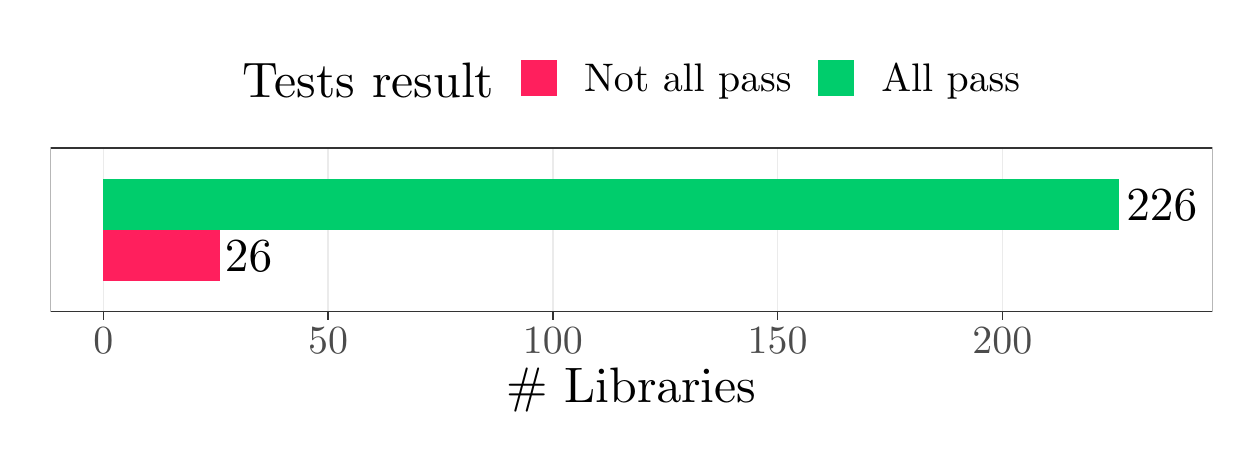
\begin{tikzpicture}[x=1pt,y=1pt]
\definecolor{fillColor}{RGB}{255,255,255}
\path[use as bounding box,fill=fillColor,fill opacity=0.00] (0,0) rectangle (433.62,144.54);
\begin{scope}
\path[clip] (  0.00,  0.00) rectangle (433.62,144.54);
\definecolor{drawColor}{RGB}{255,255,255}
\definecolor{fillColor}{RGB}{255,255,255}

\path[draw=drawColor,line width= 0.6pt,line join=round,line cap=round,fill=fillColor] (  0.00,  0.00) rectangle (433.62,144.54);
\end{scope}
\begin{scope}
\path[clip] (  8.25, 41.81) rectangle (428.12,101.14);
\definecolor{fillColor}{RGB}{255,255,255}

\path[fill=fillColor] (  8.25, 41.81) rectangle (428.12,101.14);
\definecolor{drawColor}{gray}{0.92}

\path[draw=drawColor,line width= 0.6pt,line join=round] ( 27.34, 41.81) --
	( 27.34,101.14);

\path[draw=drawColor,line width= 0.6pt,line join=round] (108.55, 41.81) --
	(108.55,101.14);

\path[draw=drawColor,line width= 0.6pt,line join=round] (189.76, 41.81) --
	(189.76,101.14);

\path[draw=drawColor,line width= 0.6pt,line join=round] (270.97, 41.81) --
	(270.97,101.14);

\path[draw=drawColor,line width= 0.6pt,line join=round] (352.19, 41.81) --
	(352.19,101.14);
\definecolor{fillColor}{RGB}{255,31,93}

\path[fill=fillColor] ( 27.34, 52.94) rectangle ( 69.57, 71.48);
\definecolor{fillColor}{RGB}{0,205,108}

\path[fill=fillColor] ( 27.34, 71.48) rectangle (394.42, 90.02);
\definecolor{drawColor}{RGB}{0,0,0}

\node[text=drawColor,anchor=base west,inner sep=0pt, outer sep=0pt, scale=  1.71] at ( 71.27, 56.33) {26};

\node[text=drawColor,anchor=base west,inner sep=0pt, outer sep=0pt, scale=  1.71] at (396.98, 74.87) {226};
\definecolor{drawColor}{gray}{0.20}

\path[draw=drawColor,line width= 0.6pt,line join=round,line cap=round] (  8.25, 41.81) rectangle (428.12,101.14);
\end{scope}
\begin{scope}
\path[clip] (  0.00,  0.00) rectangle (433.62,144.54);
\definecolor{drawColor}{gray}{0.20}

\path[draw=drawColor,line width= 0.6pt,line join=round] ( 27.34, 39.06) --
	( 27.34, 41.81);

\path[draw=drawColor,line width= 0.6pt,line join=round] (108.55, 39.06) --
	(108.55, 41.81);

\path[draw=drawColor,line width= 0.6pt,line join=round] (189.76, 39.06) --
	(189.76, 41.81);

\path[draw=drawColor,line width= 0.6pt,line join=round] (270.97, 39.06) --
	(270.97, 41.81);

\path[draw=drawColor,line width= 0.6pt,line join=round] (352.19, 39.06) --
	(352.19, 41.81);
\end{scope}
\begin{scope}
\path[clip] (  0.00,  0.00) rectangle (433.62,144.54);
\definecolor{drawColor}{gray}{0.30}

\node[text=drawColor,anchor=base,inner sep=0pt, outer sep=0pt, scale=  1.44] at ( 27.34, 26.95) {0};

\node[text=drawColor,anchor=base,inner sep=0pt, outer sep=0pt, scale=  1.44] at (108.55, 26.95) {50};

\node[text=drawColor,anchor=base,inner sep=0pt, outer sep=0pt, scale=  1.44] at (189.76, 26.95) {100};

\node[text=drawColor,anchor=base,inner sep=0pt, outer sep=0pt, scale=  1.44] at (270.97, 26.95) {150};

\node[text=drawColor,anchor=base,inner sep=0pt, outer sep=0pt, scale=  1.44] at (352.19, 26.95) {200};
\end{scope}
\begin{scope}
\path[clip] (  0.00,  0.00) rectangle (433.62,144.54);
\definecolor{drawColor}{RGB}{0,0,0}

\node[text=drawColor,anchor=base,inner sep=0pt, outer sep=0pt, scale=  1.80] at (218.18,  9.00) {\# Libraries};
\end{scope}
\begin{scope}
\path[clip] (  0.00,  0.00) rectangle (433.62,144.54);
\definecolor{fillColor}{RGB}{255,255,255}

\path[fill=fillColor] ( 72.27,112.14) rectangle (364.10,139.04);
\end{scope}
\begin{scope}
\path[clip] (  0.00,  0.00) rectangle (433.62,144.54);
\definecolor{drawColor}{RGB}{0,0,0}

\node[text=drawColor,anchor=base west,inner sep=0pt, outer sep=0pt, scale=  1.80] at ( 77.77,119.39) {Tests result};
\end{scope}
\begin{scope}
\path[clip] (  0.00,  0.00) rectangle (433.62,144.54);
\definecolor{fillColor}{RGB}{255,255,255}

\path[fill=fillColor] (177.60,119.09) rectangle (192.05,133.54);
\end{scope}
\begin{scope}
\path[clip] (  0.00,  0.00) rectangle (433.62,144.54);
\definecolor{fillColor}{RGB}{255,31,93}

\path[fill=fillColor] (178.31,119.80) rectangle (191.34,132.83);
\end{scope}
\begin{scope}
\path[clip] (  0.00,  0.00) rectangle (433.62,144.54);
\definecolor{fillColor}{RGB}{255,255,255}

\path[fill=fillColor] (285.00,119.09) rectangle (299.45,133.54);
\end{scope}
\begin{scope}
\path[clip] (  0.00,  0.00) rectangle (433.62,144.54);
\definecolor{fillColor}{RGB}{0,205,108}

\path[fill=fillColor] (285.71,119.80) rectangle (298.74,132.83);
\end{scope}
\begin{scope}
\path[clip] (  0.00,  0.00) rectangle (433.62,144.54);
\definecolor{drawColor}{RGB}{0,0,0}

\node[text=drawColor,anchor=base west,inner sep=0pt, outer sep=0pt, scale=  1.44] at (201.05,121.35) {Not all pass};
\end{scope}
\begin{scope}
\path[clip] (  0.00,  0.00) rectangle (433.62,144.54);
\definecolor{drawColor}{RGB}{0,0,0}

\node[text=drawColor,anchor=base west,inner sep=0pt, outer sep=0pt, scale=  1.44] at (308.45,121.35) {All pass};
\end{scope}
\end{tikzpicture}
